\documentclass[preview,multi,crop=false,border=1in,class=memoir]{standalone}
\usepackage{../common}

\begin{document}
\begin{preview-page}

\section{初识Erlang}

\subsection{表达式}

Erlang可以进行简单的算术运算。打开Erlang Shell,输入算术表达式和
\verb|.| 后按回车,就会显示运算结果。这个运算结果叫做表达式的值。

\begin{ErlangShellSession}
1> 1+1.
2
2> 5-2.
3
3> 2*2.
4
4> 1+2*2.
5
5> (1+2)*2.
6
6>
\end{ErlangShellSession}

\subsection{函数}

把一列数 $1,2,3,4$ 称作一个数列。这个数列共有四项,其中,第 $1$ 项为
$1$ ,第$2$ 项为 $2$ ,第 $3$ 项为 $3$ ,第 $4$ 项为 $4$ 。可以把这个数
列记作:

\begin{equation*}
a_n = \left\{
\begin{array}{l l}
1 &, n = 1 \\
2 &, n = 2 \\
3 &, n = 3 \\
4 &, n = 4 \\
\end{array} \right.
\end{equation*}

根据这个公式,可以从数列某一项的下标得到该项的值。可以用Erlang的函数来
表示这种对应关系。

\begin{SourceCode}[5]{seq1.erl}
a(1) -> 1;
a(2) -> 2;
a(3) -> 3;
a(4) -> 4.
\end{SourceCode}

把这段代码称为函数 \verb|a/1| 的定义,其中 \verb|a| 是函数 \verb|a/1|
的函数名, \verb|1| 表示函数 \verb|a/1| 只接受 \verb|1| 个参数,这里这
个参数对应数列的下标。一个函数的定义,可以由一个或者多个分句组成。多个
分句之间需要用 \verb|;| 隔开。函数定义需要以 \verb|.| 结尾。 \verb|->|
左边是分句的头, \verb|->| 右边是分句的正文。分句的正文可以由一个或者多
个表达式组成,多个表达式之间需要用 \verb|,| 隔开。把指定参数求函数的值
称为调用。

\subsection{模块}

在调用这个函数之前,需要把这几行代码保存到一个文件里。Erlang代码是按模
块组织的,每个模块会有一个对应的文件。还需要额外的几行代码来声明模块信
息。

\begin{SourceCode}{seq1.erl}
-module(seq1).

-export([a/1]).

a(1) -> 1;
a(2) -> 2;
a(3) -> 3;
a(4) -> 4.
\end{SourceCode}

\verb|-module(seq1).| 表示模块名是 \verb|seq1| ,通常,其对应源代码的文
件是 \verb|seq1.erl| 。而 \verb|-export([a/1]).| 表示,函数 \verb|a/1|
是公开的,也就是可以在其所在模块之外被调用。

\nonzeroparskip

打开Erlang Shell,输入 \verb|c(seq1).| ,按回车之后就会根据\verb|seq1|
模块的源代码(也就是文件 \verb|seq1.erl| 的内容),生成文件
\verb|seq1.beam| 。这个过程叫做编译。有了 \verb|seq1.beam| 这个文件,就
可以直接在Erlang Shell里调用 \verb|seq1| 模块里公开的函数了。需要指明模
块名,即在函数名前加上模块名 \verb|seq1| 和 \verb|:| 。

\begin{ErlangShellSession}
1> c(seq1).
{ok,seq1}
2> seq1:a(1).
1
3> seq1:a(2).
2
4> seq1:a(3).
3
5> seq1:a(4).
4
6>
\end{ErlangShellSession}

以后没有特殊说明,都假设用到的模块已经实现编译好了。

\subsection{模式}

回到函数 \verb|a/1| 的定义

\begin{SourceCode}[5]{seq1.erl}
a(1) -> 1;
a(2) -> 2;
a(3) -> 3;
a(4) -> 4.
\end{SourceCode}

Erlang在调用函数时,会按顺序逐个尝试,直到找到第一个能和传入参数匹配的
分句,对分句正文的表达式逐个求值,并以最后一个表达式的值,作为函数调用
表达式的值。假如没找到,程序就会出错。

\begin{ErlangShellSession}
1> seq1:a(5).
** exception error: no function clause matching seq1:a(5) (seq1.erl, line 5)
2>
\end{ErlangShellSession}

因为是按顺序的,所以即便有两个能匹配的,Erlang也只会用第一个。不妨在下
面增加一个分句。

\begin{SourceCode}[5]{seq2.erl}
a(1) -> 1;
a(2) -> 2;
a(3) -> 3;
a(4) -> 4;
a(4) -> 5.
\end{SourceCode}

可以看到结果仍然是4。甚至在编译时Erlang都警告说,第9行没有机会匹配。

\begin{ErlangShellSession}
1> c(seq2).
seq2.erl:9: Warning: this clause cannot match because a previous clause at line 8 always matches
{ok,seq2}
2> seq2:a(4).
4
3>
\end{ErlangShellSession}

有一个数列 $1,1,1,...$ ,这个数列有无穷项,且从第 $1$ 项开始每一项都是
$1$ ,可以记作

\begin{equation*}
b_n = 1, n = 1,2,3,...
\end{equation*}

可以用以下Erlang代码来表示这个数列。

\begin{SourceCode}[5]{seq3.erl}
b(_) -> 1.
\end{SourceCode}

\verb|_| 表示无论传入的这个参数是什么,到这里都会匹配。

\begin{ErlangShellSession}
1> seq3:b(1).
1
2> seq3:b(2).
1
3> seq3:b(3).
1
4> seq3:b(4).
1
5>
\end{ErlangShellSession}

有一个数列 $1,2,3,...$ ,这个数列有无穷项,且从第1项开始每一项的值都等
于该项下标,可以记作

\begin{equation*}
c_n = n, n = 1,2,3,...
\end{equation*}

可以用以下Erlang代码来表示这个数列。

\begin{SourceCode}[5]{seq4.erl}
c(N) -> N.
\end{SourceCode}

\verb|N| 是一个变量。变量的首字母都是大写的。在这里,\verb|N| 和
\verb|_| 的作用类似,无论传入的这个参数是什么,到这里都会匹配。不同的是,
匹配后,在分句的正文里, \verb|N| 对应的值就是当前传入参数的值。

\begin{ErlangShellSession}
1> seq4:c(1).
1
2> seq4:c(2).
2
3> seq4:c(3).
3
4> seq4:c(4).
4
5>
\end{ErlangShellSession}

回到数列 $b_n$ 。虽然,对于数列里所有下标,函数都能给出正确的结果,但是,
对于其他整数,函数却没有出错,这不是期望的结果。

\begin{ErlangShellSession}
1> seq3:b(0).
1
2> seq3:b(-1).
1
3>
\end{ErlangShellSession}

函数一个分句的头部,还可以有一个或多个用,隔开的guard,用来限制匹配的参
数的取值范围。

\begin{SourceCode}[5]{seq5.erl}
b(N) when N >= 1 -> 1.
\end{SourceCode}

加上了guard之后就会出错了。

\begin{ErlangShellSession}
1> seq5:b(0).
** exception error: no function clause matching seq5:b(0) (seq5.erl, line 5)
2>
\end{ErlangShellSession}

数列 $c_n$ ,也需要限制取值范围。

\begin{SourceCode}[5]{seq6.erl}
c(N) when N >= 1 -> N.
\end{SourceCode}

同样会出错了。

\begin{ErlangShellSession}
1> seq6:c(0).
** exception error: no function clause matching seq6:c(0) (seq6.erl, line 5)
2>
\end{ErlangShellSession}

Erlang还可以在表达式里匹配,其中一种是 \verb|case| 表达式。数列 $a_n$也
可以用下面这样的Erlang代码表示

\begin{SourceCode}[5][11]{seq7.erl}
a(N) ->
    case N of
        1 -> 1;
        2 -> 2;
        3 -> 3;
        4 -> 4
    end.
\end{SourceCode}

结果和之前的写法是一样的

\begin{ErlangShellSession}
1> seq7:a(1).
1
2> seq7:a(2).
2
3> seq7:a(3).
3
4> seq7:a(4).
4
5>
\end{ErlangShellSession}

另一种表达式, \verb|=| 右边是一个表达式,相当于是传入的参数,
\verb|=| 左边相当于函数定义里某个分句头。假如不匹配,那么就会出错。匹配
的话,这个表达式的值,就是 \verb|=| 右边表达式的值。

\begin{ErlangShellSession}
1> 1 = 1.
1
2> 1 = 1+1.
** exception error: no match of right hand side value 2
3>
\end{ErlangShellSession}

当 \verb|case| 表达式里只有一个分句,且这个分句没有使用guard。那么就可
以由这种表达式代替。我们可以用这种表达式来写测试 \cite{Armstrong:2009:unittest}。
\verb|=| 左边写期望的值, \verb|=| 右边写要测试的表达式,因为不匹配就会
出错,这样就知道哪里不符合期望了。

\begin{SourceCode}[14]{seq7.erl}
test() ->
    1 = a(1),
    2 = a(2),
    3 = a(3),
    4 = a(4),
    ok.
\end{SourceCode}

可以在一个函数里,列出所有的测试,最后一个表达式写 \verb|ok| ,这样没有出错就会
看到ok。而不需要在Erlang Shell里重复输入这些表达式了。

\begin{ErlangShellSession}
1> seq7:test().
ok
2>
\end{ErlangShellSession}

\begin{Exercise}[title={fac}, difficulty={1}]
阶乘数列 $f_n$ 的定义如下

\begin{equation*}
f_n = \left\{
\begin{array}{l l}
1              &, n = 1 \\
n \cdot f_{n-1} &, n > 1 \\
\end{array} \right.
\end{equation*}

其前 $5$ 项分别为 $1, 2, 6, 24, 120$

在 \verb|fac| 模块里,定义一个公开函数 \verb|f/1| 来表示这个数列。

每个练习都会有一个名字,紧跟在练习编号以及难度后面的就是练习的名字了。
比如现在这个练习的名字是fac。

在每个章节的目录下,都有一个 \verb|exercise| 模块。里面定义了
\verb|check/1| 函数,可以对练习的代码进行一些基本的检查。请把练习的名字
作为参数去调用这个函数。

假如你的代码没问题,结果就会是 \verb|ok| 。

\begin{ErlangShellSession}
1> exercise:check(fac).
ok
2>
\end{ErlangShellSession}

\verb|check/1| 函数里对应的定义如下

\begin{SourceCode}[5][11]{exercise.erl}
check(fac) ->
    1 = fac:f(1),
    2 = fac:f(2),
    6 = fac:f(3),
    24 = fac:f(4),
    120 = fac:f(5),
    ok;
\end{SourceCode}

以后没有特殊说明,就表示可以用 \verb|check/1| 来检查。

\end{Exercise}

\begin{Answer}
\begin{SourceCode}{fac.erl}
-module(fac).

-export([f/1]).

f(1) ->
    1;
f(N)
  when N > 1->
    N * f(N-1).
\end{SourceCode}
\end{Answer}

\nonzeroparskip

\begin{Exercise}[title={fib}, difficulty={1}]
在 \verb|fac| 模块里,定义一个公开函数 \verb|f/1| 来表示Fibonacci数列。

Fibonacci数列 $f_n$ 的定义如下

\begin{equation*}
f_n = \left\{
\begin{array}{l l}
1              &, n = 1 \\
1              &, n = 2 \\
f_{n-2} + f_{n-1} &, n > 2 \\
\end{array} \right.
\end{equation*}

其前 $5$ 项分别为 $1, 1, 2, 3, 5$

\begin{SourceCode}[12][18]{exercise.erl}
check(fib) ->
    1 = fib:f(1),
    1 = fib:f(2),
    2 = fib:f(3),
    3 = fib:f(4),
    5 = fib:f(5),
    ok.
\end{SourceCode}
\end{Exercise}

\begin{Answer}
\begin{SourceCode}{fib.erl}
-module(fib).

-export([f/1]).

f(1) ->
    1;
f(2) ->
    1;
f(N)
  when N > 2->
    f(N-2) + f(N-1).
\end{SourceCode}
\end{Answer}

\subsection{数据类型}

\verb|ok| 是什么?Erlang不仅能进行整数运算,还有别的数据类型。
\verb|ok| 就是一个类型为 \verb|atom()| 的数据。可以简单认为一个
\verb|atom()| 就是一连串小写字母。当且仅当每个位置上的字母都相同的时候,
才认为两个 \verb|atom()| 相同。

\begin{ErlangShellSession}
1> a = a.
a
2> a = b.
** exception error: no match of right hand side value b
3> a = aa.
** exception error: no match of right hand side value aa
4>
\end{ErlangShellSession}

那 \verb|case| 和 \verb|end| 呢? 这两个是用来表示这中间是一个 \verb|case| 表达式,都是Erlang的保留字。实际上, \verb|atom()| 必须在两个 \verb|'| 之间输入。只不过,假如一个 \verb|atom()| 是小写字母开头的,不包含特殊字符,而且不是保留字,输入时就可以省略前后两个 \verb|'| 。

\begin{ErlangShellSession}
1> case.
* 1: syntax error before: '.'
1> 'case'.
'case'
2> a = 'a'.
a
3>
\end{ErlangShellSession}

\nonzeroparskip

假设存在一个 $8 \times 8$ 的棋盘,横坐标是1到8,纵坐标也是1到8。

\begin{figure}[hbt]
\centering
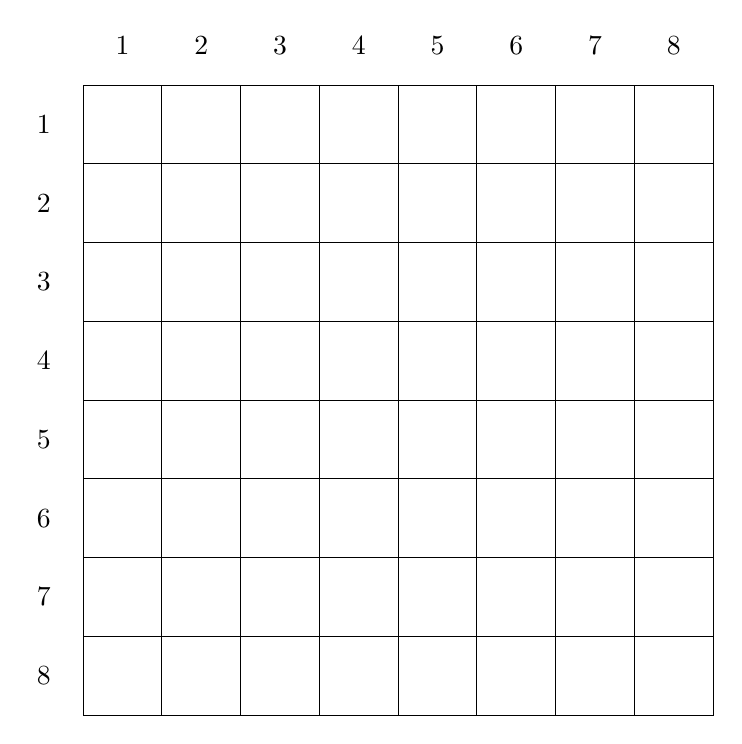
\begin{tikzpicture}
\foreach \x in {1,2,...,8} {
  \draw (\x,9) node{\x};
}

\foreach \y in {1,2,...,8} {
  \draw (0,9-\y) node{\y};
}

\foreach \x in {1,2,...,8}
\foreach \y in {1,...,8} {
  \draw (\x,\y) +(-.5,-.5) rectangle ++(.5,.5);
}
\end{tikzpicture}
\end{figure}

可以用一个 \verb|tuple()| 表示这个棋盘上一个格子的坐标。比如,
\verb|{1,2}| 表示横坐标为1,纵坐标为2的格子。\verb|tuple()| 可以有零个、
一个或者多个元素。只有当每个元素都相同的时候,才认为是相同的
\verb|tuple()| 。

\begin{ErlangShellSession}
1> {} = {}.
{}
2> {1} = {}.
** exception error: no match of right hand side value {}
3> {1} = {1}.
{1}
4> {1} = {1,1}.
** exception error: no match of right hand side value {1,1}
5> {1,1} = {1,{1}}.
** exception error: no match of right hand side value {1,{1}}
6>
\end{ErlangShellSession}

可以用 \verb|up|, \verb|down|, \verb|left|, \verb|right| 这四个
\verb|atom()| 来表示上下左右四个方向。定义 \verb|move/2| 函数来根据当前
坐标计算棋子移动一格之后的坐标。

\begin{figure}[hbt]
\centering
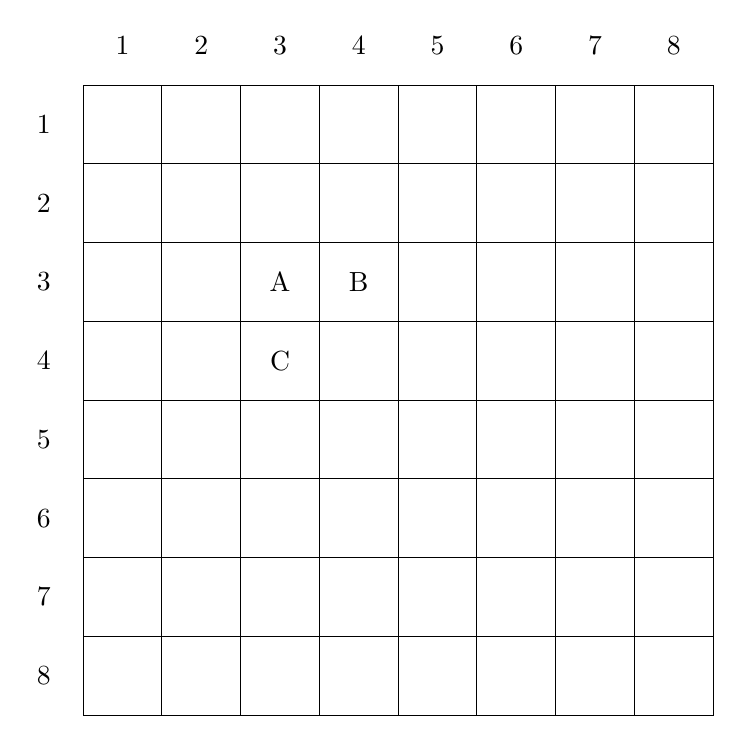
\begin{tikzpicture}
\foreach \x in {1,2,...,8} {
  \draw (\x,9) node{\x};
}

\foreach \y in {1,2,...,8} {
  \draw (0,9-\y) node{\y};
}

\foreach \x in {1,2,...,8}
\foreach \y in {1,...,8} {
  \draw (\x,\y) +(-.5,-.5) rectangle ++(.5,.5);
}

\draw(3,6) node{A};
\draw(4,6) node{B};
\draw(3,5) node{C};
\end{tikzpicture}
\end{figure}

如上图所示,A往右移一格就到B,B往左边移一格就到A,A往下移一格就到C,C往
上移一格就到A。

\begin{SourceCode}[25][32]{board.erl}
test(move) ->
    A = {3,3},
    B = {4,3},
    C = {3,4},
    B = move(right, A),
    A = move(left, B),
    C = move(down, A),
    A = move(up, C);
\end{SourceCode}

分别用 \verb|X|, \verb|Y| 表示横坐标和纵坐标,往左就是把横坐标减一,往
右就是把横坐标加一,往上就是把纵坐标减一,往下就是把纵坐标加一。

\begin{SourceCode}[5][16]{board.erl}
move(left, {X,Y})
  when X > 1, X =< 8 ->
    {X-1, Y};
move(right, {X,Y})
  when X >= 1, X < 8 ->
    {X+1, Y};
move(up, {X,Y})
  when Y > 1, Y =< 8 ->
    {X, Y-1};
move(down, {X,Y})
  when Y >= 1, Y < 8 ->
    {X, Y+1}.
\end{SourceCode}


\begin{Exercise}[title={board1},difficulty={1}]
停止
\end{Exercise}

\begin{Exercise}[title={board2},difficulty={1}]
到另一边
\end{Exercise}

\begin{Exercise}[title={board3}, difficulty={1}]
move\_n
\end{Exercise}

\nonzeroparskip

用一个 \verb|list()| 来表示多步移动的方向。\verb|list()| 和
\verb|tuple()| 相似,都是多个元素按顺序组合起来的。\verb|tuple()| 适合
表示和同一个事物相关的多个数据,比如一个格子的横坐标和纵坐标。而
\verb|list()| 适合表示很多个同类的数据,比如多个方向,多个坐标。

\begin{SourceCode}[33][35]{board.erl}
test(moves) ->
    {4,1} = moves([right,right,right], {1,1}),
    {1,4} = moves([down,down,down], {1,1}).
\end{SourceCode}

用 \verb|list()| 是因为, \verb|list()| 可以方便地取出前几个元素,比如,
\verb#[A1,A2,A3|B]# 就表示一个 \verb|list()| 的前3个元素,分别为
\verb|A1|, \verb|A2|, \verb|A3|。把剩余的元素按顺序组合起来的
\verb|list()| 和 \verb|B| 相同。

\begin{ErlangShellSession}
1> [a, b] = [a|[b]].
[a,b]
2> [a, b, c] = [a,b|[c]].
[a,b,c]
3> [a] = [a|[]].
[a]
4> [a,b|_] = [a,b,c].
[a,b,c]
5> [a,b|_] = [a,b,c,d].
[a,b,c,d]
6>
\end{ErlangShellSession}

若 \verb|list()| 为空,说明不需要再移动了,那么起始坐标就是最终坐标。否
则,取出第一个方向,把按此移动一步后的坐标作为新的起始坐标,再来计算。

\begin{SourceCode}[19][22]{board.erl}
moves([], From) ->
    From;
moves([H|T], From) ->
    moves(T, move(H, From)).
\end{SourceCode}

\begin{Exercise}[title={length}, difficulty={1}]
\end{Exercise}

\begin{Exercise}[title={sum}, difficulty={1}]
\end{Exercise}

\end{preview-page}
\end{document}
